%===================================================================================
\chapter{Code Organization}\label{s:organization}
%===================================================================================

%----------------------------------
\section{SUNDIALS organization}\label{ss:sun_org}
%----------------------------------
% This is a shared SUNDIALS TEX file with description of
% the SUNDIALS organization
%
The family of solvers referred to as {\sundials} consists of the solvers
{\cvode} (for ODE systems), {\kinsol} (for nonlinear algebraic
systems), and {\ida} (for differential-algebraic systems).  In addition,
{\sundials} also includes variants of {\cvode} and {\ida} with sensitivity analysis 
capabilities (using either forward or adjoint methods): {\cvodes} and {\idas},
respectively.

The various solvers of this family share many subordinate modules.
For this reason, it is organized as a family, with a directory
structure that exploits that sharing (see Fig. \ref{f:sunorg}).
\begin{figure}
\subfigure[High-level diagram]
{\centerline{\psfig{figure=sunorg1.eps,width=\textwidth}}}
\subfigure[Directory structure of the source tree]
{\centerline{\psfig{figure=sunorg2.eps,width=\textwidth}}}
\caption {Organization of the SUNDIALS suite}\label{f:sunorg}
\end{figure}
The following is a list of the solver packages presently available:
\begin{itemize}

\item {\cvode},  
  a solver for stiff and nonstiff ODEs $dy/dt = f(t,y)$;

\item {\cvodes},
  a solver for stiff and nonstiff ODEs
  with sensitivity analysis capabilities;

\item {\ida},
  a solver for differential-algebraic systems $F(t,y,y^\prime) = 0$;

\item {\idas},
  a solver for differential-algebraic systems
  with sensitivity analysis capabilities;

\item {\kinsol}, 
  a solver for nonlinear algebraic systems $F(u) = 0$.

\end{itemize}


%----------------------------------
\section{IDAS organization}\label{ss:idas_org}
%----------------------------------

\index{IDAS@{\idas}!package structure}
The {\idas} package is written in the ANSI {\CC} language. The following
summarizes the basic structure of the package, although knowledge
of this structure is not necessary for its use.

The overall organization of the {\idas} package is shown in Figure
\ref{f:idasorg}.
\begin{figure}
{\centerline{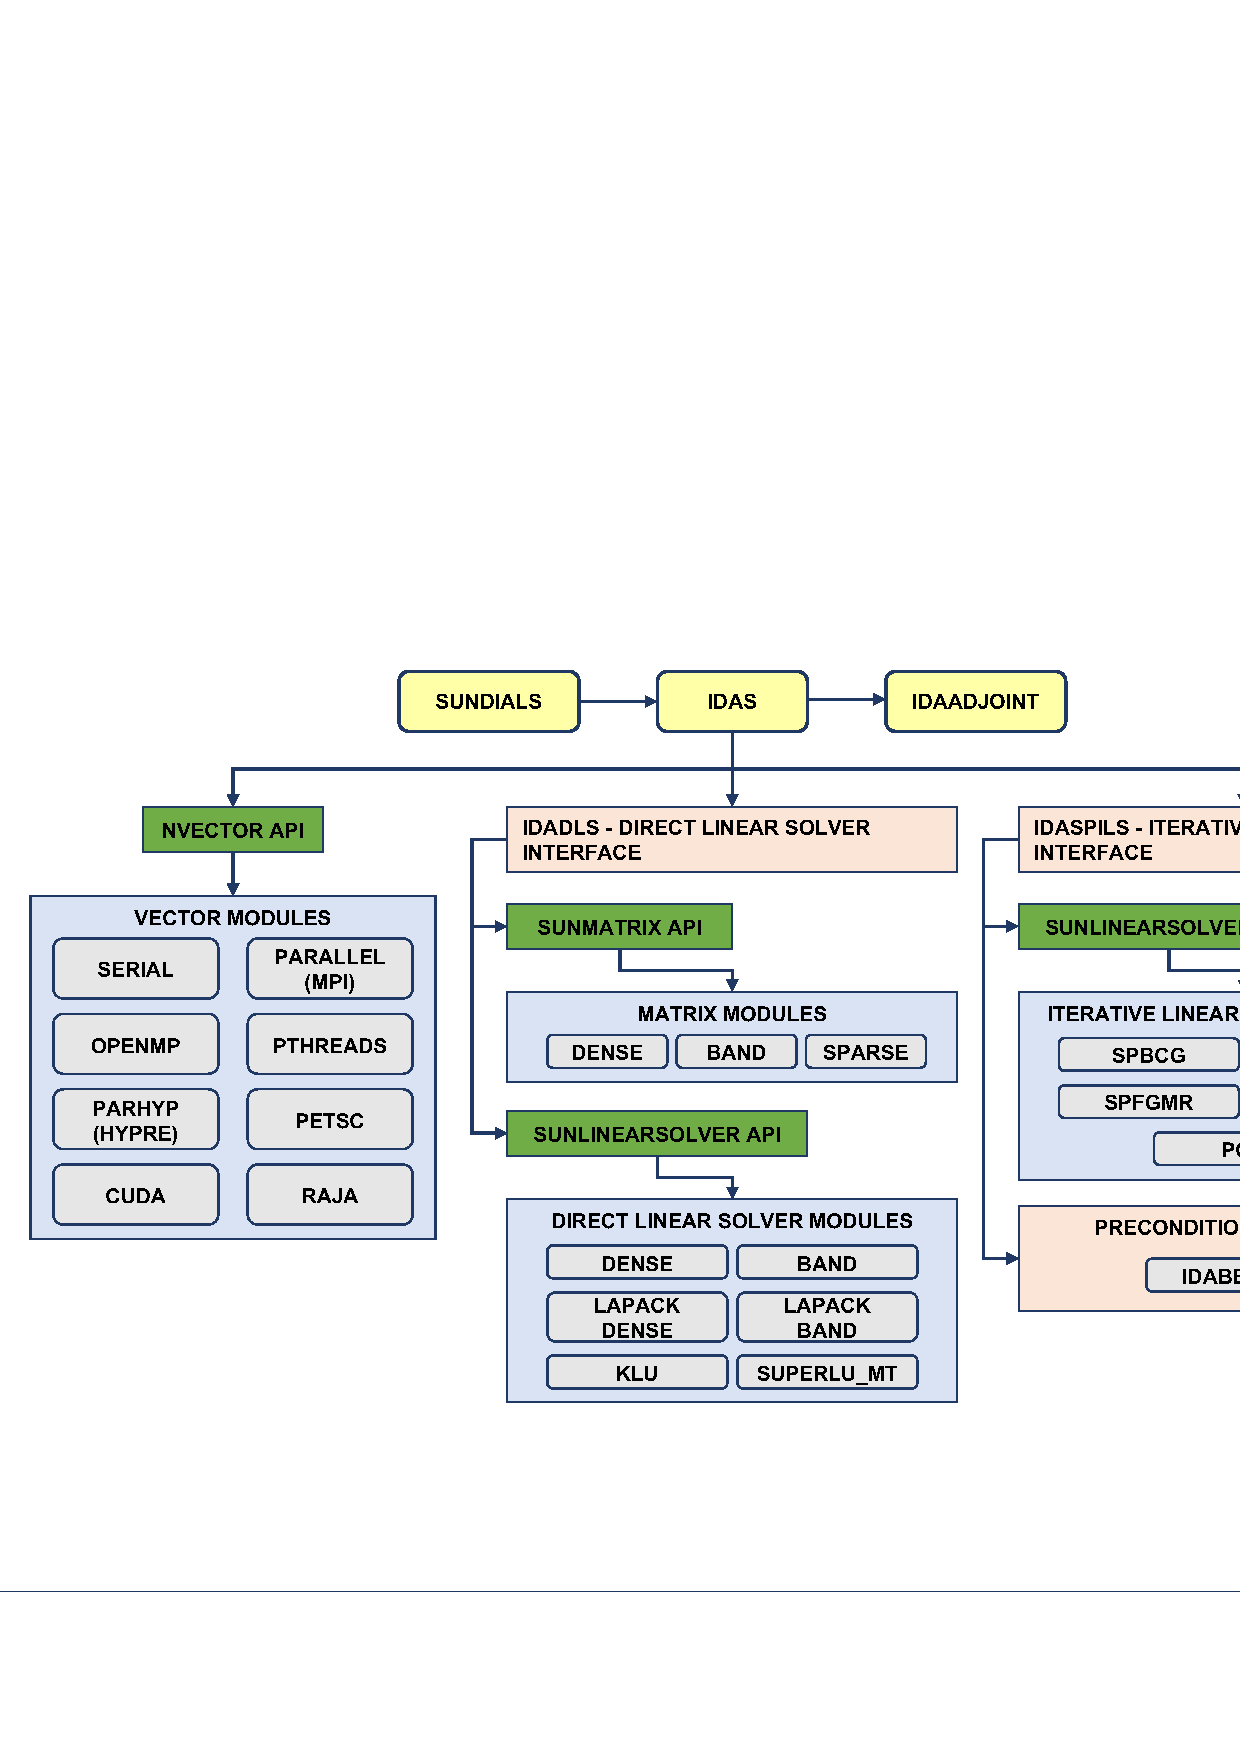
\includegraphics[width=\textwidth]{idasorg}}}
\caption [Overall structure diagram of the {\idas} package]
{Overall structure diagram of the {\idas} package.
  Modules specific to {\idas} are distinguished by rounded boxes, while 
  generic solver and auxiliary modules are in square boxes.
  Note that the direct linear solvers using Lapack implementations are not 
  explicitly represented.
  Note also that the KLU and SuperLU\_MT support 
  is through interfaces
  to packages.  Users will need to download and compile those packages independently.}
\label{f:idasorg}
\end{figure}
The central integration module, implemented in the files \id{idas.h},
\id{idas\_impl.h}, and \id{idas.c}, deals with the evaluation of integration 
coefficients, the Newton iteration process, estimation of local error,
selection of stepsize and order, and interpolation to user output
points, among other issues.  Although this module contains logic for
the basic Newton iteration algorithm, it has no knowledge of the
method being used to solve the linear systems that arise.  For any
given user problem, one of the linear system modules is specified, and
is then invoked as needed during the integration. 

In addition, if forward sensitivity analysis is turned on, the main module 
will integrate the forward sensitivity equations simultaneously with the original
IVP. The sensitivity variables may be included in the local error control
mechanism of the main integrator.
\index{forward sensitivity analysis!correction strategies}
{\idas} provides two different strategies for dealing with the correction
stage for the sensitivity variables: \Id{IDA\_SIMULTANEOUS} \Id{IDA\_STAGGERED}
(see \S\ref{ss:fwd_sensi}).
The {\idas} package includes an algorithm for the approximation of the
sensitivity equations residuals by difference quotients, but the user has
the option of supplying these residual functions directly.

\index{adjoint sensitivity analysis!implementation in {\idas}|(}
The adjoint sensitivity module (file \id{idaa.c}) provides the infrastructure needed for the 
backward integration of any system of DAEs which depends on the solution 
of the original IVP, in particular the adjoint system and any quadratures required
in evaluating the gradient of the objective functional.  This module deals with
the setup of the checkpoints, the interpolation of the forward solution during
the backward integration, and the backward integration of the adjoint equations.
\index{adjoint sensitivity analysis!implementation in {\idas}|)}

\index{IDAS@{\idas} linear solvers!list of|(} 
At present, the package includes the following seven {\idas} linear algebra
modules, organized into two families. The {\em direct} family of linear
solvers provides solvers for the direct solution of linear systems with
dense or banded matrices and includes:
\begin{itemize} 
\item {\idadense}: LU factorization and backsolving with dense matrices
  (using either an internal implementation or Blas/Lapack); 
\item {\idaband}: LU factorization and backsolving with banded matrices
  (using either an internal implementation or Blas/Lapack); 
\item {\idaklu}: LU factorization and backsolving with
  compressed-sparse-column (CSC) matrices using the KLU linear solver
  library \cite{DaPa:10,KLU_site} (KLU to be downloaded and compiled by user independent 
  of {\ida});
\item {\idasuperlumt}: LU factorization and backsolving with
  compressed-sparse-column (CSC) matrices using the threaded
  SuperLU\_MT linear solver library \cite{Li:05,DGL:99,SuperLUMT_site} 
  (SuperLU\_MT to be downloaded and compiled by user independent 
  of {\ida}).
\end{itemize}
The {\em spils} family of linear solvers provides scaled preconditioned
iterative linear solvers and includes:
\begin{itemize} 
\item {\idaspgmr}: scaled preconditioned GMRES method;
\item {\idaspbcg}: scaled preconditioned Bi-CGStab method;
\item {\idasptfqmr}: scaled preconditioned TFQMR method.
\end{itemize}
The set of linear solver modules distributed with {\idas} is intended to be expanded in the
future as new algorithms are developed.
Note that users wishing to employ KLU or 
SuperLU\_MT will need to download and install these 
libraries independent of {\sundials}.
{\sundials} provides only the interfaces between itself and these libraries.
\index{IDAS@{\idas} linear solvers!list of|)} 

In the case of the direct methods {\idadense} and {\idaband}
the package includes an algorithm for the approximation of the Jacobian by difference
quotients, but the user also has the option of supplying the Jacobian
(or an approximation to it) directly. When using the sparse direct
linear solvers {\idaklu} and {\idasuperlumt} the user must supply a
routine for the Jacobian (or an approximation to it) in CSC format,
since standard difference quotient approximations do not leverage the
inherent sparsity of the problem. In the case of the Krylov iterative methods 
{\idaspgmr}, {\idaspbcg}, and {\idasptfqmr}, the package includes an algorithm for
the approximation by difference quotients of the product between the Jacobian matrix
and a vector of appropriate length. Again, the user has the option of providing
a routine for this operation.
When \index{preconditioning!setup and solve phases} using any of the Krylov
methods, the user must supply the preconditioning in two phases: 
a setup phase (preprocessing of Jacobian data) and a solve phase.
While\index{preconditioning!advice on} there is no default
choice of preconditioner analogous to the difference quotient
approximation in the direct case, the references
\cite{BrHi:89, Byr:92}, together with
the example and demonstration programs included with {\idas}, offer
considerable assistance in building preconditioners.

\index{IDAS@{\idas} linear solvers!implementation details|(} 
Each {\idas} linear solver module consists of five routines, devoted to
(1) memory allocation and initialization, (2) setup of the matrix data
involved, (3) solution of the system, (4) monitoring performance,
and (5) freeing of memory.  
The setup and solution phases are separate because the evaluation of
Jacobians and preconditioners is done only periodically during the
integration, as required to achieve convergence. The call list within
the central {\idas} module to each of the five associated functions is
fixed, thus allowing the central module to be completely independent
of the linear system method.
\index{IDAS@{\idas} linear solvers!implementation details|)} 

These modules are also decomposed in another way.
\index{generic linear solvers!use in {\idas}|(} 
Each of the linear solver modules ({\idadense} etc.) consists of an
interface built on top of a generic linear system solver ({\dense}
etc.).  The interface deals with the use of the particular method in
the {\idas} context, whereas the generic solver is independent of the
context.  While some of the generic linear system solvers ({\dense},
{\band}, {\spgmr}, {\spbcg}, and {\sptfqmr}) were written with
{\sundials} in mind, they are intended to be usable anywhere as
general-purpose solvers.  This separation also allows for any generic
solver to be replaced by an improved version, with no necessity to
revise the {\idas} package elsewhere. 
\index{generic linear solvers!use in {\idas}|)}

{\idas} also provides a preconditioner module,
{\idabbdpre}, that works in conjunction with {\nvecp} and generates a 
preconditioner that is a block-diagonal matrix with each block being 
a band matrix.

All state information used by {\idas} to solve a given problem is saved
in a structure, and a pointer to that structure is returned to the
user.  There is no global data in the {\idas} package, and so, in this
respect, it is reentrant. State information specific to the linear
solver is saved in a separate structure, a pointer to which resides in
the {\idas} memory structure. The reentrancy of {\idas} was motivated
by the situation where two or more problems are solved by
intermixed calls to the package from one user program.

